%%%%%%%%%%%%%%%%%%%%%%%%%%%%%%%%%%%%%%%%%%%%%%%%%%%%%%%%
%   |------------------------------------------|       %
%   | Web App embebida en dispositivos móviles |       %
%   |  para la gestión de registros sobre la   |       %
%   |   contaminación de afluentes y ríos.     |       %
%   |                                          |       %
%   |          Proyecto de graduación          |       %
%   |__________________________________________|       %
%                                                      %
%   Autores                                            %
%   -------                                            %
%                                                      %
% * Bruno, Ricardo Hugo (CX 1409686)                   %
%     rburnount@gmail.com                              %
% * Gomez Veliz, Kevin Shionen (CX 1411828)            %
%     ing.gomezvelizkevin@gmail.com                    %
%                                                      %
%   Tutor                                              %
%   -------                                            %
%                                                      %
% * Ing. Cohen, Daniel Eduardo                         %
%        dcohen.tuc@gmail.com                          %
%                                                      %
%   Cotutor                                            %
%   -------                                            %
%                                                      %
% * Ing. Nieto, Luis Eduardo                           %
%        lnieto@herrera.unt.edu.ar                     %
%                                                      %
%                                                      %
%%%%%%%%%%%%%%%%%%%%%%%%%%%%%%%%%%%%%%%%%%%%%%%%%%%%%%%%

\chapter{Disciplina de Diseño}
\label{chap:disenio}

Por el Principio de Pareto\footnote{Cuando se habla de los costes de desarrollo de software enunciarse de la siguiente manera: ``El 80\% del esfuerzo de desarrollo (en tiempo y recursos) produce el 20\% del código, mientras que el 80\% restante es producido con tan sólo un 20\% del esfuerzo''}, se hicieron los diagramas relevantes. Como se procura tener homogeneidad en la implementación de las clases, basta un solo diagrama de cada tipo para una clase, para describir también el comportamiento de las otras clases.

\section{Descripción Textual de Casos de Uso}

%#############################################################################
%#   
%#   Caso de uso 1
%#
%#############################################################################

\subsection{Caso de Uso UC1: Autenticar}

\begin{framed}

%\noindent\hline

\subsubsection{Resumen:} Este caso de uso permite a los usuarios autenticarse con el nombre de usuario y contraseña de manera que el sistema les permita realizar operaciones.


\subsubsection{Actores:} Usuario (primario). Servidor (en adelante S secundario)

\subsubsection{Personal Involucrado y Metas:}

\emph{Usuario:} quiere que el sistema lo reconozca como tal, así pueda realizar las transacciones con la aplicación de un modo seguro y personalizado.

\emph{Servidor:} requiere identificar confiablemente a sus usuarios de manera de satisfacer sus intereses en cuanto a seguridad, accesos a su cuenta personal y datos privados. 

\subsubsection{Precondiciones:} 
El usuario está registrado 

\subsubsection{Poscondiciones:} 
Se identifica y autentica al usuario. Se conocen sus datos personales y opciones de personalización.

\subsubsection{Escenario Principal: }

\begin{enumerate}
    \item El usuario ejecuta la aplicación móvil (en adelante AM) en su teléfono celular. 
    \item AM solicita al usuario su identificador y contraseña. 
    \item El usuario ingresa su identificador y contraseña. 
    \item AM solicita a S la validación del usuario. 
    \item S valida al usuario y comunica sus datos personales. 
    \item AM da la bienvenida al usuario. 
\end{enumerate}

\subsubsection{Flujos Alternativos: }

%El  comando alternativo está definido en el documento principal. Es un paragraph con salto de línea
\alternativo{A1: El sistema encuentra algún fallo para comunicarse con S}
La secuencia A1 comienza en el punto 4 del escenario principal. 
\begin{enumerate}
    %Comienza a partir del 5° item
    \setcounter{enumi}{4}
    \item AM informa al usuario el problema de conexión a través de un mensaje por la pantalla. 
\end{enumerate}
El escenario vuelve al punto 4. 


\alternativo{A2: Nombre de usuario inexistente}
La secuencia A2 comienza en el punto 4 del escenario principal.
\begin{enumerate}
    \setcounter{enumi}{4}
        \item S comunica que el nombre de usuario es inexistente. 
\end{enumerate}
El escenario vuelve al punto 2. 


\alternativo{A3: Nombre de usuario existe pero contraseña inválida }
La secuencia A2 comienza en el punto 4 del escenario principal. 
\begin{enumerate}
    \setcounter{enumi}{4}
    \item S comunica que la contraseña es inválida. 
\end{enumerate}
El escenario vuelve al punto 2. 


\subsubsection{Requisitos de Interfaz de Usuario para todos los casos de uso: }
Teléfono celular con SO Android y pantalla táctil 

\subsubsection{Requisitos No-Funcionales para todos los casos de uso:}
\emph{Tiempo de respuesta:} la interfaz debe responder dentro de un tiempo máximo de 10 segundos en una velocidad efectiva de conexión con el servidor a través de 3G.

\emph{Disponibilidad:} debe poder accederse en un régimen 24x7.
%}}
\end{framed}


%#############################################################################
%#   
%#   Caso de uso 2
%#
%#############################################################################


\subsection{Caso de Uso UC2: Registrar}

\begin{framed}

%\noindent\hline

\subsubsection{Resumen:} Este caso de uso permite a los usuarios registrarse como usuarios de la aplicación, permitiendo introducir sus datos y preferencias personales


\subsubsection{Actores:} Usuario (primario). Servidor (en adelante S secundario)

\subsubsection{Personal Involucrado y Metas:}

\emph{Usuario:} quiere transformarse en un usuario del sistema, así pueda realizar las transacciones con la aplicación de un modo seguro y personalizado.

\emph{Servidor:} quiere registrar la mayor cantidad de usuarios posibles y que el proceso sea lo más rápido y seguro posible. 

\subsubsection{Precondiciones:} 
El usuario no está registrado en la aplicación. 

\subsubsection{Poscondiciones:} 
Se registra al usuario como usuario de la aplicación. El usuario puede realizar operaciones en la aplicación.

\subsubsection{Escenario Principal: }

\begin{enumerate}
    \item El usuario ejecuta la AM en su teléfono celular y decide registrarse. 
    \item AM muestra un formulario de carga donde ingresa sus datos personales y su nombre de usuario y contraseña.
    \item AM solicita a S el registro del usuario. 
    \item S registra al usuario y lo informa a AM. 
    \item AM da la bienvenida al usuario
   
\end{enumerate}

\subsubsection{Flujos Alternativos: }

%El  comando alternativo está definido en el documento principal. Es un paragraph con salto de línea
\alternativo{A1:El sistema encuentra algún fallo para comunicarse con S}
La secuencia A1 comienza en el punto 3 del escenario principal. 
\begin{enumerate}
    %Comienza a partir del 5° item
    \setcounter{enumi}{3}
    \item AM informa al usuario el problema de conexión a través de un mensaje por la pantalla.
\end{enumerate}
El escenario vuelve al punto 3. 


\alternativo{A2: Nombre de usuario existente}
La secuencia A2 comienza en el punto 3 del escenario principal.
\begin{enumerate}
    \setcounter{enumi}{3}
        \item S comunica que el nombre de usuario es existente.
\end{enumerate}
El escenario vuelve al punto 2. 


\alternativo{A3: Contraseña inválida o no coincide con la confirmación }
La secuencia A2 comienza en el punto 3 del escenario principal. 
\begin{enumerate}
    \setcounter{enumi}{3}
    \item S comunica que la contraseña es inválida. 
\end{enumerate}
El escenario vuelve al punto 2. 

\alternativo{A4: dirección de correo electrónico existente }
La secuencia A2 comienza en el punto 3 del escenario principal. 
\begin{enumerate}
    \setcounter{enumi}{3}
    \item S comunica que la dirección de correo electrónico es existente. 
\end{enumerate}
El escenario vuelve al punto 2. 

%}}
\end{framed}

%#############################################################################
%#   
%#   Caso de uso 3
%#
%#############################################################################

\subsection{Caso de Uso UC3: Crear Tienda}

\begin{framed}

%\noindent\hline

\subsubsection{Resumen:} Este caso de uso permite al vendedor crear una tienda de manera que el sistema le permita realizar transacciones y operaciones sobre sus productos.


\subsubsection{Actores:} Vendedor (primario). S (secundario)

\subsubsection{Personal Involucrado y Metas:}

\emph{Vendedor:} quiere que el sistema lo reconozca como tal, así pueda realizar las transacciones a través del sitio, y la administración de sus productos de un modo seguro y personalizado.

\emph{Servidor:} requiere identificar confiablemente a sus usuarios vendedores de manera de satisfacer sus intereses en cuanto a seguridad, productos publicados y datos privados. 

\subsubsection{Precondiciones:} 
Los usuarios deben estar autenticados en AM. 

\subsubsection{Poscondiciones:} 
Se registra una nueva tienda en el sistema con los datos básicos necesarios para realizar ventas.

\subsubsection{Escenario Principal: }

\begin{enumerate}
    \item El vendedor selecciona la opción para crear tienda. 
    \item AM solicita al vendedor a través de un formulario los datos básicos requeridos para la creación de la tienda.
    \item El vendedor completa el formulario y presiona un botón para finalizar.
    \item AM envía de manera segura los datos a S para que sean validados.
    \item S valida los datos, realiza la creación la tienda y envía una confirmación.
    \item AM informa al usuario que la operación se realizó exitosamente.
\end{enumerate}

\subsubsection{Flujos Alternativos: }

%El  comando alternativo está definido en el documento principal. Es un paragraph con salto de línea
\alternativo{A1:el sistema encuentra algún fallo para comunicarse con S}
La secuencia A1 comienza en el punto 4 del escenario principal. 
\begin{enumerate}
    %Comienza a partir del 5° item
    \setcounter{enumi}{4}
    \item AM informa al usuario el problema de conexión a través de un mensaje por la pantalla.
\end{enumerate}
El escenario vuelve al punto 4.

%}}
\end{framed}

%#############################################################################
%#   
%#   Caso de uso 4
%#
%#############################################################################


\subsection{Caso de Uso UC4: Editar Tienda}

\begin{framed}

%\noindent\hline

\subsubsection{Resumen:} Este caso de uso permite al vendedor editar los datos de su tienda.


\subsubsection{Actores:} Vendedor (primario). S (secundario)

\subsubsection{Personal Involucrado y Metas:}

\emph{Vendedor:} quiere editar los datos de su tienda.

\emph{Servidor:} requiere mantener actualizados los datos del vendedor.

\subsubsection{Precondiciones:} 
El vendedor debe estar autenticado en AM. 

\subsubsection{Poscondiciones:} 
Se registran los cambios de los datos de la tienda en el servidor.

\subsubsection{Escenario Principal: }

\begin{enumerate}
    \item El vendedor selecciona la opción para editar tienda. 
    \item AM solicita al vendedor a través de un formulario los datos de la tienda que pueden ser modificados o mantenidos.
    \item El vendedor completa el formulario y presiona un botón para finalizar.
    \item AM envía de manera segura los datos a S para que sean validados.
    \item S valida los datos, realiza la actualización y envía una confirmación.
    \item AM informa al usuario que la operación se realizó exitosamente.
\end{enumerate}

\subsubsection{Flujos Alternativos: }

%El  comando alternativo está definido en el documento principal. Es un paragraph con salto de línea
\alternativo{A1:El sistema encuentra algún fallo para comunicarse con S}
La secuencia A1 comienza en el punto 4 del escenario principal.
\begin{enumerate}
    %Comienza a partir del 5° item
    \setcounter{enumi}{4}
    \item AM informa al usuario el problema de conexión a través de un mensaje por la pantalla.
\end{enumerate}
El escenario vuelve al punto 4.

%}}
\end{framed}

%#############################################################################
%#   
%#   Caso de uso 5
%#
%#############################################################################


\subsection{Caso de Uso UC5: Editar Perfil}

\begin{framed}

%\noindent\hline

\subsubsection{Resumen:} Este caso de uso permite al usuario editar los datos de su perfil.


\subsubsection{Actores:} Usuario(primario). S (secundario)

\subsubsection{Personal Involucrado y Metas:}

\emph{Usuario:} quiere editar los datos de su perfil.

\emph{Servidor:} requiere mantener actualizados los datos del usuario.

\subsubsection{Precondiciones:} 
El usuario debe estar autenticado en AM. 

\subsubsection{Poscondiciones:} 
Se registran los cambios de los datos de perfil en el servidor.

\subsubsection{Escenario Principal: }

\begin{enumerate}
    \item El usuario selecciona la opción para editar perfil. 
    \item AM solicita al usuario a través de un formulario los datos del perfil de usuario que pueden ser modificados o mantenidos.
    \item El usuario completa el formulario y presiona un botón para finalizar.
    \item AM envía de manera segura los datos a S para que sean validados.
    \item S valida los datos, realiza la actualización y envía una confirmación.
    \item AM informa al usuario que la operación se realizó exitosamente.
\end{enumerate}

\subsubsection{Flujos Alternativos: }

%El  comando alternativo está definido en el documento principal. Es un paragraph con salto de línea
\alternativo{A1:el sistema encuentra algún fallo para comunicarse con S}
La secuencia A1 comienza en el punto 4 del escenario principal.
\begin{enumerate}
    %Comienza a partir del 5° item
    \setcounter{enumi}{4}
    \item AM informa al usuario el problema de conexión a través de un mensaje por la pantalla.
\end{enumerate}
El escenario vuelve al punto 4.

%}}
\end{framed}

%#############################################################################
%#   
%#   Caso de uso 6
%#
%#############################################################################


\subsection{Caso de Uso UC6: Crear Producto}

\begin{framed}

%\noindent\hline

\subsubsection{Resumen:} Este caso de uso permite al vendedor crear un producto de manera que el sistema le permita ofrecerlo a la venta.


\subsubsection{Actores:} Vendedor (primario). S (secundario)

\subsubsection{Personal Involucrado y Metas:}

\emph{Vendedor:} quiere ofrecer sus productos a través del sistema.

\emph{Servidor:} requiere obtener la información de los  productos de manera que sea posible ofrecérselo a los compradores.

\subsubsection{Precondiciones:} 
El vendedor debe estar autenticados en AM. 

\subsubsection{Poscondiciones:} 
Se crea un nuevo producto en el sistema.

\subsubsection{Escenario Principal: }

\begin{enumerate}
    \item El vendedor selecciona la opción para crear producto. 
    \item AM solicita al vendedor a través de un formulario los datos básicos requeridos para la creación del producto.
    \item El vendedor completa el formulario y presiona un botón para finalizar.
    \item AM envía de manera segura los datos a S para que sean validados.
    \item S valida los datos, realiza la creación del producto y envía una confirmación.
    \item AM informa al usuario que la operación se realizó exitosamente.
\end{enumerate}

\subsubsection{Flujos Alternativos: }

%El  comando alternativo está definido en el documento principal. Es un paragraph con salto de línea
\alternativo{A1:el sistema encuentra algún fallo para comunicarse con S}
La secuencia A1 comienza en el punto 4 del escenario principal.
\begin{enumerate}
    %Comienza a partir del 5° item
    \setcounter{enumi}{4}
    \item AM informa al vendedor el problema de conexión a través de un mensaje por la pantalla.
\end{enumerate}
El escenario vuelve al punto 4.

%}}
\end{framed}

%#############################################################################
%#   
%#   Caso de uso 7
%#
%#############################################################################


\subsection{Caso de Uso UC7: Editar Producto}

\begin{framed}

%\noindent\hline

\subsubsection{Resumen:} Este caso de uso permite al vendedor editar los datos de uno de sus productos.


\subsubsection{Actores:} Vendedor (primario). S (secundario)

\subsubsection{Personal Involucrado y Metas:}

\emph{Vendedor:} quiere ofrecer sus productos a través del sistema.

\emph{Servidor:} requiere obtener la información de los  productos de manera que sea posible ofrecérselo a los compradores.

\subsubsection{Precondiciones:} 
El vendedor debe estar autenticados en AM. 

\subsubsection{Poscondiciones:} 
Se registran los cambios de los datos del producto en el servidor.

\subsubsection{Escenario Principal: }

\begin{enumerate}
    \item El vendedor selecciona la opción para editar producto. 
    \item AM solicita al vendedor a través de un formulario los datos del producto que pueden ser modificados o mantenidos.
    \item El vendedor completa el formulario y presiona un botón para finalizar.
    \item AM envía de manera segura los datos a S para que sean validados.
    \item S valida los datos, realiza la actualización y envía una confirmación.
    \item AM informa al usuario que la operación se realizó exitosamente.
\end{enumerate}

\subsubsection{Flujos Alternativos: }

%El  comando alternativo está definido en el documento principal. Es un paragraph con salto de línea
\alternativo{A1:el sistema encuentra algún fallo para comunicarse con S}
La secuencia A1 comienza en el punto 4 del escenario principal.
\begin{enumerate}
    %Comienza a partir del 5° item
    \setcounter{enumi}{4}
    \item AM informa al vendedor el problema de conexión a través de un mensaje por la pantalla.
\end{enumerate}
El escenario vuelve al punto 4.

%}}
\end{framed}

%#############################################################################
%#   
%#   Caso de uso 8
%#
%#############################################################################


\subsection{Caso de Uso UC8: Eliminar Producto}

\begin{framed}

%\noindent\hline

\subsubsection{Resumen:} Este caso de uso permite al vendedor eliminar un producto de la tienda.


\subsubsection{Actores:} Vendedor (primario). S (secundario)

\subsubsection{Personal Involucrado y Metas:}

\emph{Vendedor:} quiere eliminar un producto de su tienda.

\emph{Servidor:} elimina al producto.

\subsubsection{Precondiciones:} 
El vendedor debe estar autenticados en AM. 

\subsubsection{Poscondiciones:} 
Se elimina el producto de la tienda.

\subsubsection{Escenario Principal: }

\begin{enumerate}
    \item El vendedor selecciona la opción para eliminar el producto. 
    \item AM solicita al vendedor que confirme que quiere eliminar el producto.
    \item El vendedor presiona un botón para confirmar.
    \item AM envía de manera segura la solicitud a S para que sean validados.
    \item S valida la solicitud, realiza el cambio de estado en el producto y envía una confirmación.
    \item AM informa al usuario que la operación se realizó exitosamente.
\end{enumerate}

\subsubsection{Flujos Alternativos: }

%El  comando alternativo está definido en el documento principal. Es un paragraph con salto de línea
\alternativo{A1:el sistema encuentra algún fallo para comunicarse con S}
La secuencia A1 comienza en el punto 4 del escenario principal.
\begin{enumerate}
    %Comienza a partir del 5° item
    \setcounter{enumi}{4}
    \item AM informa al vendedor el problema de conexión a través de un mensaje por la pantalla.
\end{enumerate}
El escenario vuelve al punto 4.

%}}
\end{framed}

%#############################################################################
%#   
%#   Caso de uso 9
%#
%#############################################################################


\subsection{Caso de Uso UC9: Buscar Producto}

\begin{framed}

%\noindent\hline

\subsubsection{Resumen:} Este caso de uso permite a un usuario realizar una búsqueda de productos.


\subsubsection{Actores:} Usuario (primario). S (secundario)

\subsubsection{Personal Involucrado y Metas:}

\emph{Usuario:} quiere obtener los productos que coincidan con un determinado criterio de búsqueda

\emph{Servidor:} quiere ofrecer al usuario los productos que mejor se ajustan a su búsqueda.

\subsubsection{Poscondiciones:} 
Se obtiene un listado de productos que cumplen con la condición de búsqueda.

\subsubsection{Escenario Principal: }

\begin{enumerate}
    \item El usuario ingresa el texto que se buscará.  
    \item El usuario presiona un botón para comenzar la búsqueda.
    \item AM envía la solicitud de búsqueda a S
    \item S verifica los productos que cumplen con el criterio buscado
    \item S retorna el listado de productos
    \item AM muestra el listado al usuario
\end{enumerate}

\subsubsection{Flujos Alternativos: }

%El  comando alternativo está definido en el documento principal. Es un paragraph con salto de línea
\alternativo{A1:el sistema encuentra algún fallo para comunicarse con S}
La secuencia A1 comienza en el punto 3 del escenario principal.
\begin{enumerate}
    %Comienza a partir del 5° item
    \setcounter{enumi}{4}
    \item AM informa al usuario el problema de conexión a través de un mensaje por la pantalla.
\end{enumerate}
El escenario vuelve al punto 3.

%}}
\end{framed}

%#############################################################################
%#   
%#   Caso de uso 10
%#
%#############################################################################

\subsection{Caso de Uso UC10: Comprar Producto}

\begin{framed}

%\noindent\hline

\subsubsection{Resumen:} Este caso de uso permite a un comprador realizar la compra de un producto.


\subsubsection{Actores:} Comprador (primario). Vendedor y S (secundarios)

\subsubsection{Personal Involucrado y Metas:}

\emph{Comprador:} quiere realizar la compra del producto en el que está interesado.

\emph{Vendedor:} quiere que la venta se realice sin inconvenientes y de manera sencilla.

\emph{Servidor:} quiere que la operación de compra se realice de manera segura y todos los datos relevantes sean almacenados correctamente.


\subsubsection{Precondiciones:} 
Los usuarios deben estar autenticados en AM.

\subsubsection{Poscondiciones:} 
Se registra la compra

\subsubsection{Escenario Principal: }

\begin{enumerate}
    \item El comprador selecciona la opción para comprar el producto.  
    \item El comprador selecciona la cantidad que desea comprar
    \item El comprador presiona un botón para confirmar la compra
    \item AM envía la solicitud de compra a S
    \item S verifica la solicitud y registra la compra
    \item AM informa al comprador que la compra se realizó correctamente
    \item S envía una notificación al vendedor informándole la compra 
    \item El vendedor contacta al comprador para que acuerden las condiciones de la compra y la entrega de los productos.
\end{enumerate}

\subsubsection{Flujos Alternativos: }

%El  comando alternativo está definido en el documento principal. Es un paragraph con salto de línea
\alternativo{A1:el sistema encuentra algún fallo para comunicarse con S}
La secuencia A1 comienza en el punto 4 del escenario principal.
\begin{enumerate}
    %Comienza a partir del 5° item
    \setcounter{enumi}{4}
    \item AM informa al comprador el problema de conexión a través de un mensaje por la pantalla.
\end{enumerate}
El escenario vuelve al punto 4.

%}}
\end{framed}

%#############################################################################
%#   
%#   Caso de uso 11
%#
%#############################################################################

\subsection{Caso de Uso UC11: Listar compras realizadas}

\begin{framed}

%\noindent\hline

\subsubsection{Resumen:} Este caso de uso permite a un comprador listar la información de todas las compras que realizó.


\subsubsection{Actores:} Comprador (primario). S (secundarios)

\subsubsection{Personal Involucrado y Metas:}

\emph{Comprador:} quiere visualizar de manera completa la información de las compras realizadas.

\emph{Servidor:} quiere que el comprador pueda ver la información relacionada con sus operaciones de manera segura.


\subsubsection{Precondiciones:} 
El comprador debe estar autenticado en AM.

\subsubsection{Poscondiciones:} 
Se muestra un listado de compras realizadas

\subsubsection{Escenario Principal: }

\begin{enumerate}
    \item El comprador selecciona la opción para listar las compras realizadas.  
    \item AM envía la solicitud a S
    \item S envía los datos necesarios para generar el listado a AM
    \item AM muestra el listado al comprador
    
\end{enumerate}

\subsubsection{Flujos Alternativos: }

%El  comando alternativo está definido en el documento principal. Es un paragraph con salto de línea
\alternativo{A1:el sistema encuentra algún fallo para comunicarse con S}
La secuencia A1 comienza en el punto 2 del escenario principal.
\begin{enumerate}
    %Comienza a partir del 5° item
    \setcounter{enumi}{2}
    \item AM informa al usuario el problema de conexión a través de un mensaje por la pantalla.
\end{enumerate}
El escenario vuelve al punto 2.

%}}
\end{framed}

%#############################################################################
%#   
%#   Caso de uso 12
%#
%#############################################################################


\subsection{Caso de Uso UC12: Listar ventas realizadas}

\begin{framed}

%\noindent\hline

\subsubsection{Resumen:} Este caso de uso permite a un vendedor listar la información de todas las ventas que realizó.


\subsubsection{Actores:} Vendedor (primario). S (secundarios)

\subsubsection{Personal Involucrado y Metas:}

\emph{Vendedor:} quiere visualizar de manera completa la información de las ventas realizadas.

\emph{Servidor:} quiere que el vendedor pueda ver la información relacionada con sus operaciones de manera segura.


\subsubsection{Precondiciones:} 
El vendedor debe estar autenticado en AM.

\subsubsection{Poscondiciones:} 
Se muestra un listado de compras realizadas

\subsubsection{Escenario Principal: }

\begin{enumerate}
    \item El vendedor selecciona la opción para listar las ventas realizadas  
    \item AM envía la solicitud a S
    \item S envía los datos necesarios para generar el listado a AM
    \item AM muestra el listado al vendedor
    
\end{enumerate}

\subsubsection{Flujos Alternativos: }

%El  comando alternativo está definido en el documento principal. Es un paragraph con salto de línea
\alternativo{A1:el sistema encuentra algún fallo para comunicarse con S}
La secuencia A1 comienza en el punto 2 del escenario principal.
\begin{enumerate}
    %Comienza a partir del 5° item
    \setcounter{enumi}{2}
    \item AM informa al usuario el problema de conexión a través de un mensaje por la pantalla.
\end{enumerate}
El escenario vuelve al punto 2.

%}}
\end{framed}

%#############################################################################
%#   
%#   Caso de uso 13
%#
%#############################################################################

\subsection{Caso de Uso UC13: Contactar Usuario}

\begin{framed}

\subsubsection{Resumen:}Este caso de uso permite a un usuario ponerse en contacto con otro.


\subsubsection{Actores:} Usuario remitente (primario). Usuario destinatario (secundario)

\subsubsection{Personal Involucrado y Metas:}

\emph{Usuario remitente:} quiere poder comunicarse con otro usuario de la aplicación.

\emph{Usuario destinatario:} quiere poder recibir las consultas que otros usuarios puedan realizarle. 


\subsubsection{Precondiciones:} 
El usuario remitente cuenta con una aplicación de correo electrónico y una cuenta configurada en su teléfono celular.

\subsubsection{Poscondiciones:} 
Se envía el mensaje al usuario destinatario a través de e-mail.

\subsubsection{Escenario Principal: }

\begin{enumerate}
    \item El Usuario remitente selecciona la opción para contactar con el Usuario destinatario.
    \item AM redirige al usuario remitente a una aplicación de gestión de correo electrónico instalada en el dispositivo, y completa la dirección destino con el e-mail del Usuario destinatario.
    \item El Usuario remitente completa el mensaje y realiza el envío
        
\end{enumerate}

\end{framed}

\section{Diagrama de Clases de Diseño}

\begin{figure}[H]
  \centering
    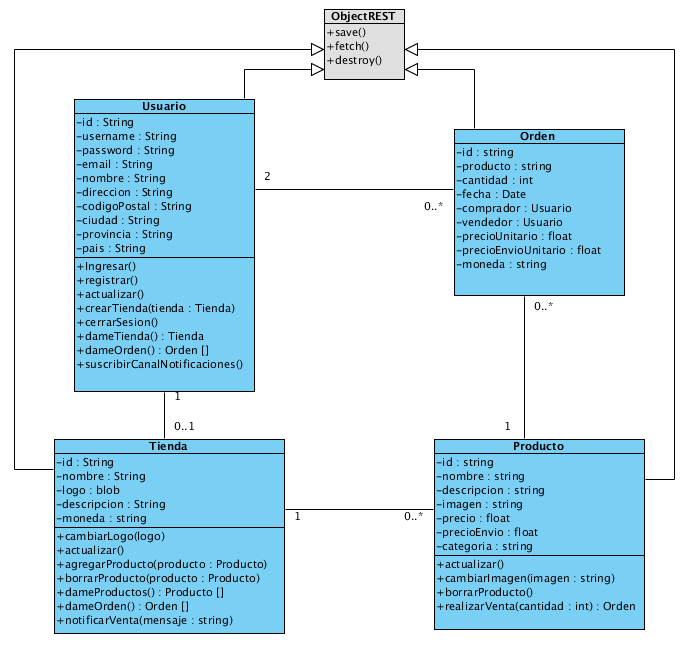
\includegraphics[width=1\textwidth]{imagenes/disenio/clases-disenio.png}
        %%Me parece que queda mejor sin el hfill
        %\hfill
    \label{fig:diagrama-clases-disenio}
\end{figure}

\section{Diagramas de Secuencia}

\subsection{Autenticar}
\begin{figure}[H]
  \centering
    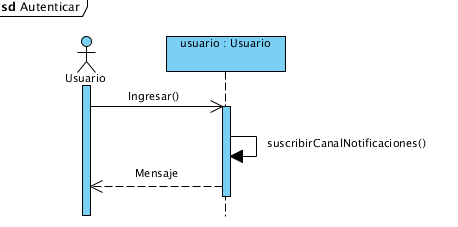
\includegraphics{imagenes/disenio/secuencia-autenticar.png}
        %%Me parece que queda mejor sin el hfill
        %\hfill
    \label{fig:diagrama-secuencia-autenticar}
\end{figure}


\subsection{Registrar}
\begin{figure}[H]
  \centering
    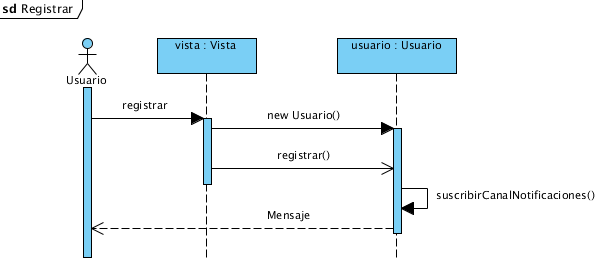
\includegraphics{imagenes/disenio/secuencia-registrar.png}
        %%Me parece que queda mejor sin el hfill
        %\hfill
    \label{fig:diagrama-secuencia-registrar}
\end{figure}

\subsection{Crear Tienda}
\begin{figure}[H]
  \centering
    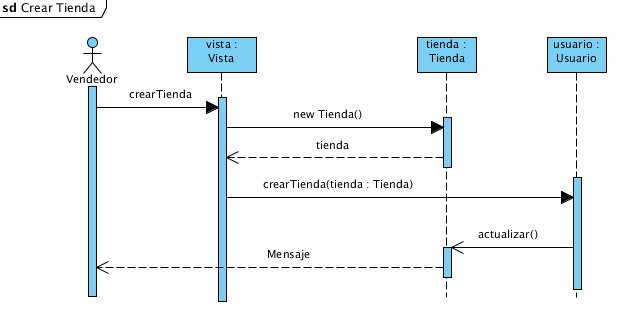
\includegraphics{imagenes/disenio/secuencia-crear-tienda.png}
        %%Me parece que queda mejor sin el hfill
        %\hfill
    \label{fig:diagrama-secuencia-crear-tienda}
\end{figure}

\subsection{Agregar Producto}
\begin{figure}[H]
  \centering
    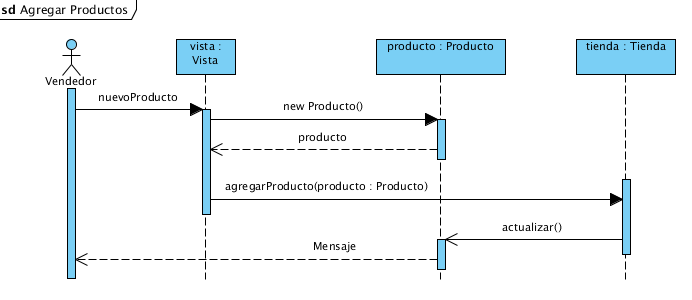
\includegraphics[width=1\textwidth]{imagenes/disenio/secuencia-agregar-producto.png}
        %%Me parece que queda mejor sin el hfill
        %\hfill
    \label{fig:diagrama-secuencia-agregar-producto}
\end{figure}

\subsection{Comprar Producto}
\begin{figure}[H]
  \centering
    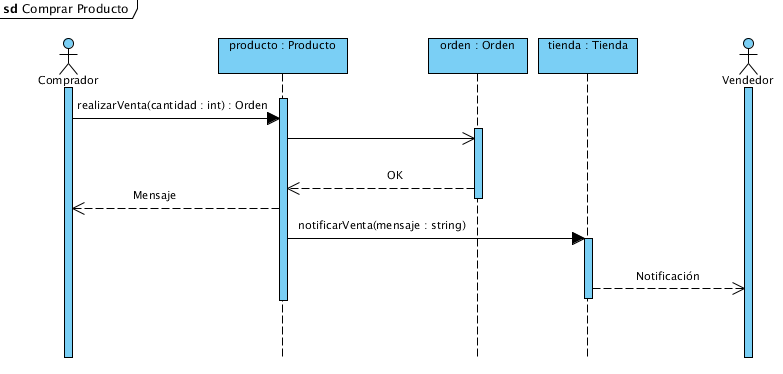
\includegraphics[width=1\textwidth]{imagenes/disenio/secuencia-comprar-producto.png}
        %%Me parece que queda mejor sin el hfill
        %\hfill
    \label{fig:diagrama-secuencia-comprar-producto}
\end{figure}

\section{Interfaz de Usuario}

\begin{figure}[H]
  \centering
    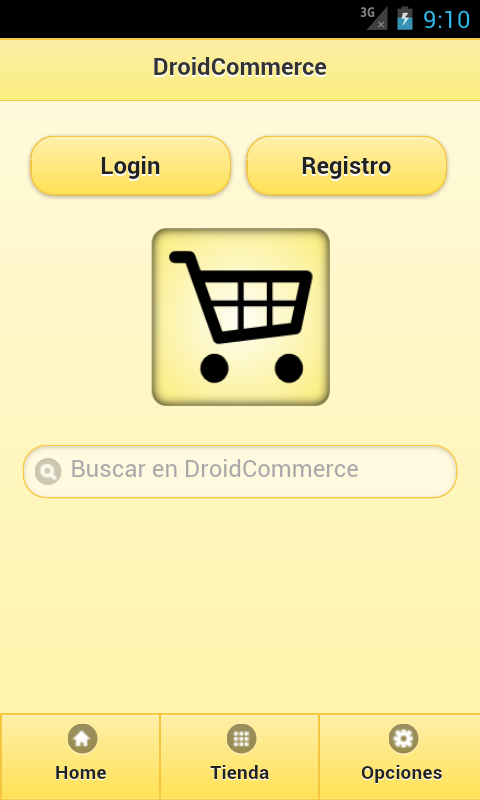
\includegraphics[width=0.6\textwidth]{imagenes/capturas/home.png}
        %%Me parece que queda mejor sin el hfill
        %\hfill
        \caption{Pantalla inicial}
    \label{fig:home}
\end{figure}

\begin{figure}
  \centering
    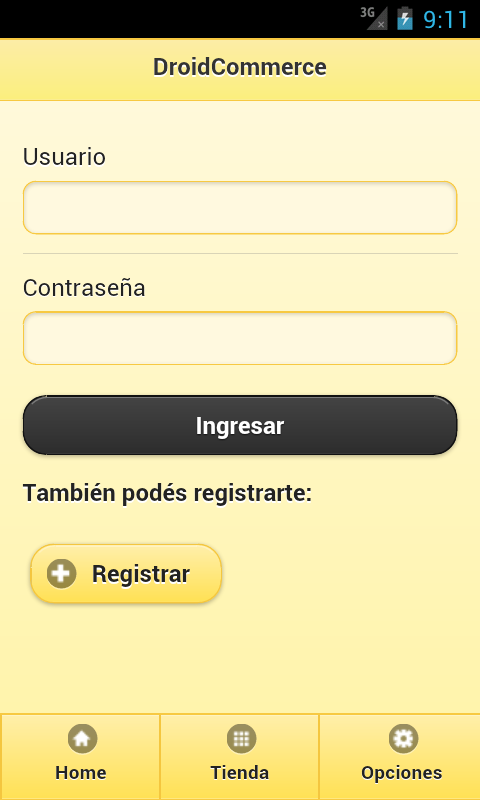
\includegraphics[width=0.6\textwidth]{imagenes/capturas/login.png}
        %%Me parece que queda mejor sin el hfill
        %\hfill
        \caption{Pantalla de login}
    \label{fig:login}
\end{figure}

\begin{figure}
  \centering
    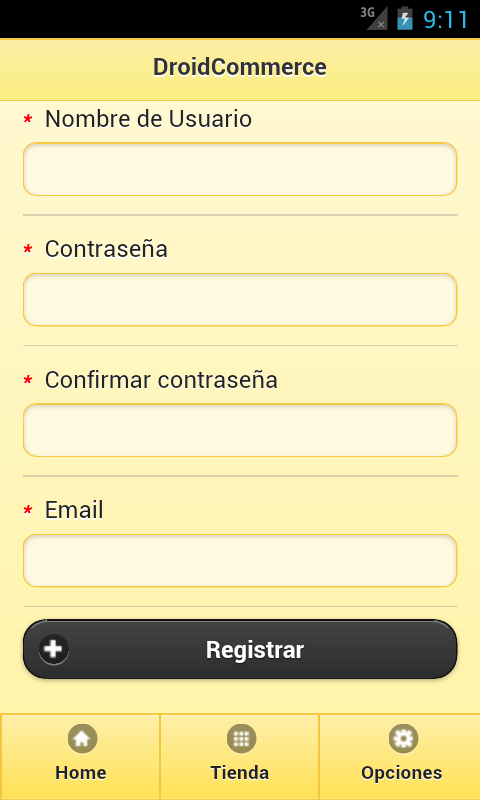
\includegraphics[width=0.6\textwidth]{imagenes/capturas/registro2.png}
        %%Me parece que queda mejor sin el hfill
        %\hfill
        \caption{Pantalla de registro}
    \label{fig:login}
\end{figure}

\begin{figure}
  \centering
    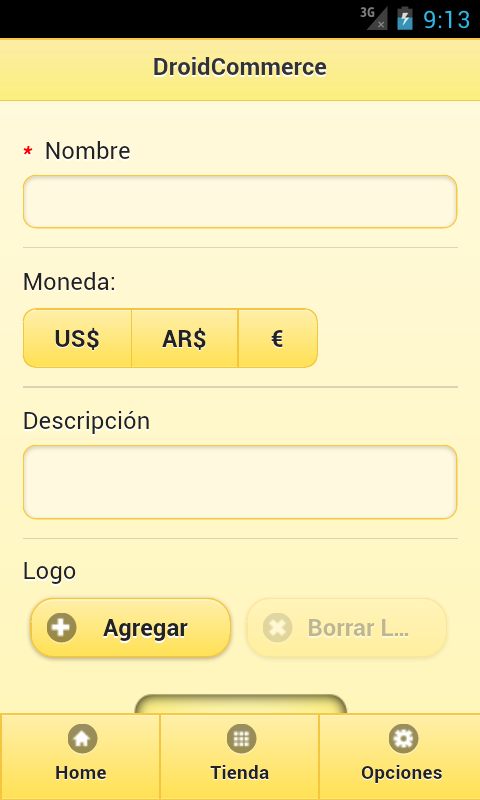
\includegraphics[width=0.6\textwidth]{imagenes/capturas/crear-tienda1.png}
        %%Me parece que queda mejor sin el hfill
        %\hfill
        \caption{Pantalla de creación de tienda, parte superior}
    \label{fig:crear-tienda-1}
\end{figure}

\begin{figure}
  \centering
    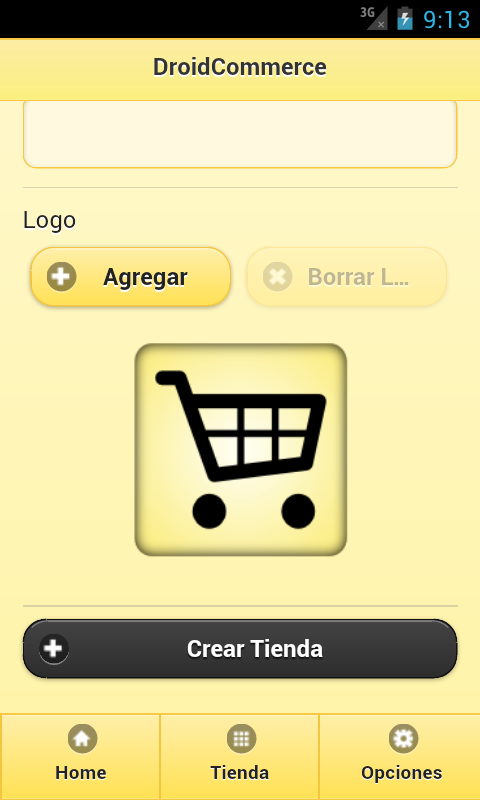
\includegraphics[width=0.6\textwidth]{imagenes/capturas/crear-tienda2.png}
        %%Me parece que queda mejor sin el hfill
        %\hfill
        \caption{Pantalla de creación de tienda, parte inferior}
    \label{fig:crear-tienda-2}
\end{figure}

\begin{figure}
  \centering
    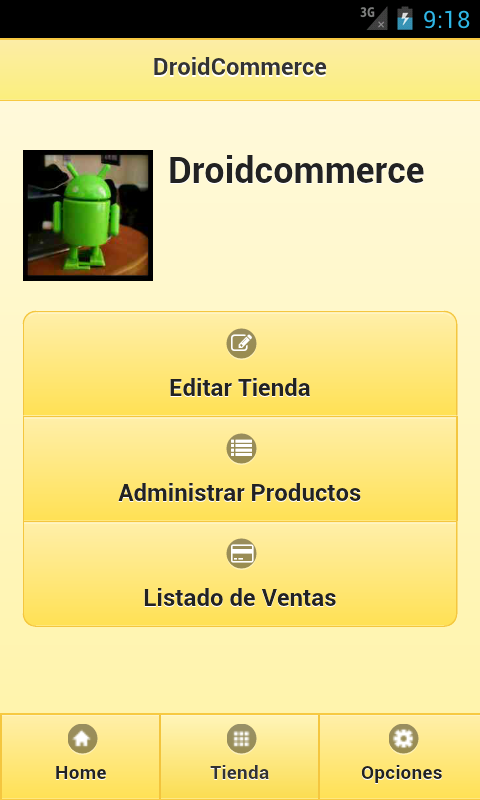
\includegraphics[width=0.6\textwidth]{imagenes/capturas/administracion-tienda.png}
        %%Me parece que queda mejor sin el hfill
        %\hfill
        \caption{Pantalla de administración de la tienda}
    \label{fig:admin-tienda}
\end{figure}


\begin{figure}
  \centering
    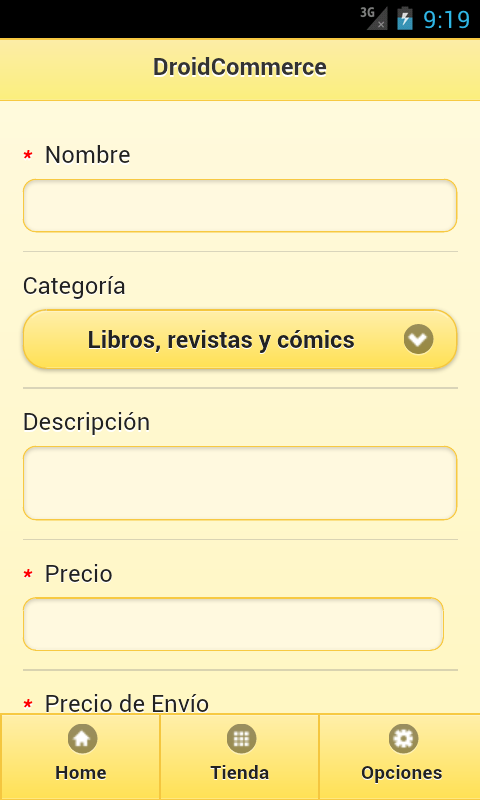
\includegraphics[width=0.6\textwidth]{imagenes/capturas/crear-producto1.png}
        %%Me parece que queda mejor sin el hfill
        %\hfill
        \caption{Pantalla de creación de producto, parte superior}
    \label{fig:crear-producto-1}
\end{figure}

\begin{figure}
  \centering
    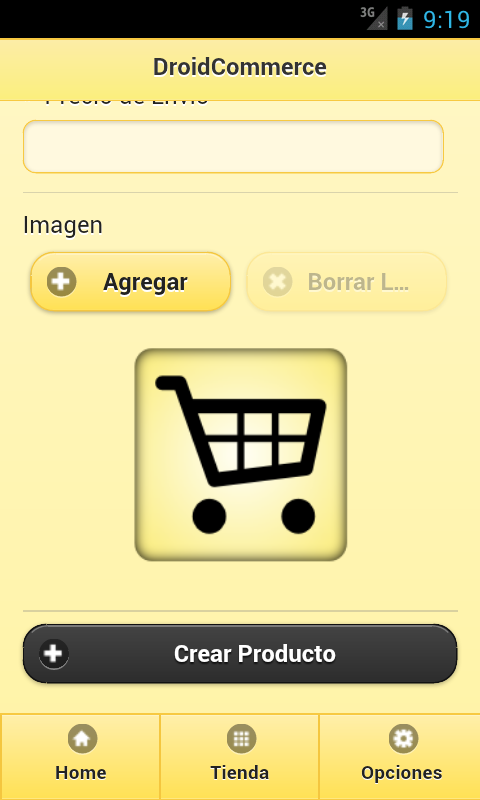
\includegraphics[width=0.6\textwidth]{imagenes/capturas/crear-producto2.png}
        %%Me parece que queda mejor sin el hfill
        %\hfill
        \caption{Pantalla de creación de producto, parte inferior}
    \label{fig:crear-producto2}
\end{figure}

\begin{figure}
  \centering
    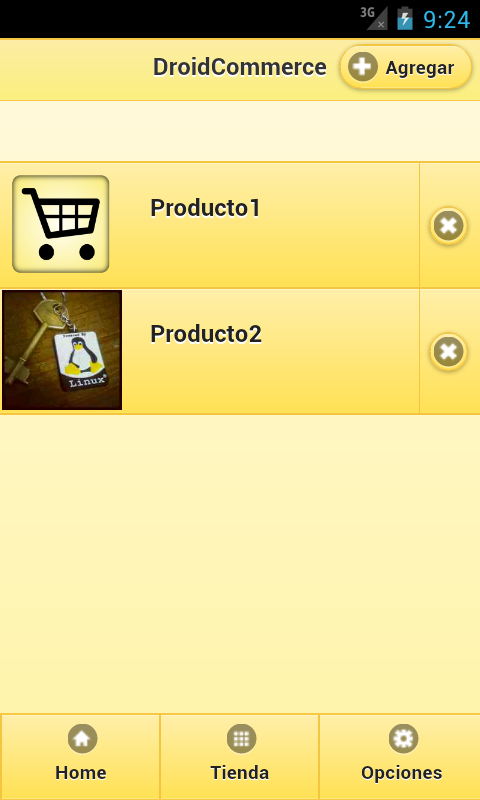
\includegraphics[width=0.6\textwidth]{imagenes/capturas/administracion-productos.png}
        %%Me parece que queda mejor sin el hfill
        %\hfill
        \caption{Pantalla de administración de productos}
    \label{fig:administrar-productos}
\end{figure}
\begin{figure}
  \centering
    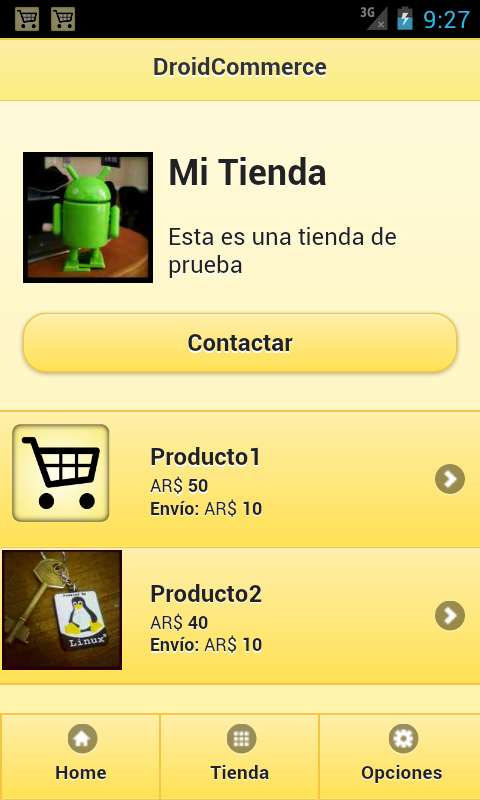
\includegraphics[width=0.6\textwidth]{imagenes/capturas/vista-tienda.png}
        %%Me parece que queda mejor sin el hfill
        %\hfill
        \caption{Pantalla de tienda}
    \label{fig:tienda}
\end{figure}

\begin{figure}
  \centering
    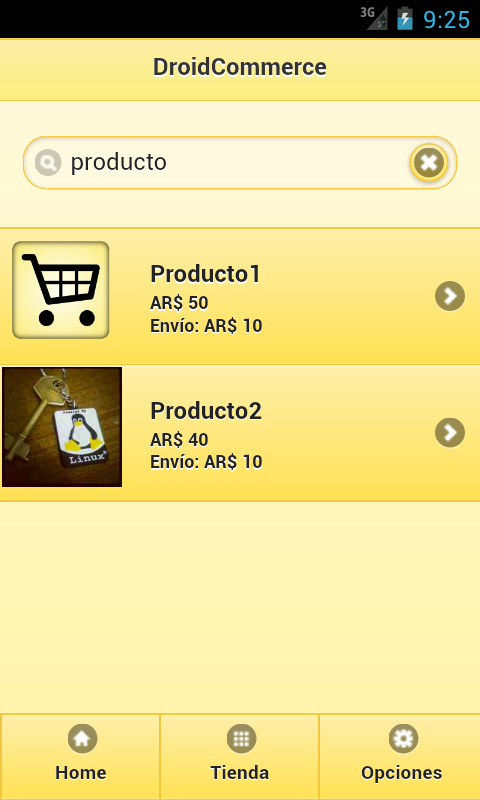
\includegraphics[width=0.6\textwidth]{imagenes/capturas/busqueda.png}
        %%Me parece que queda mejor sin el hfill
        %\hfill
        \caption{Pantalla de resultados de la búsqueda de productos}
    \label{fig:busqueda}
\end{figure}

\begin{figure}
  \centering
    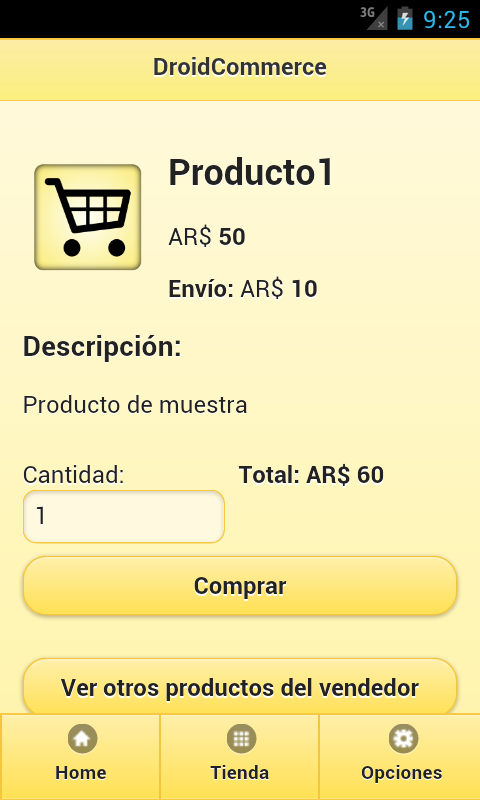
\includegraphics[width=0.6\textwidth]{imagenes/capturas/pagina-producto.png}
        %%Me parece que queda mejor sin el hfill
        %\hfill
        \caption{Pantalla de producto}
    \label{fig:producto}
\end{figure}

\begin{figure}
  \centering
    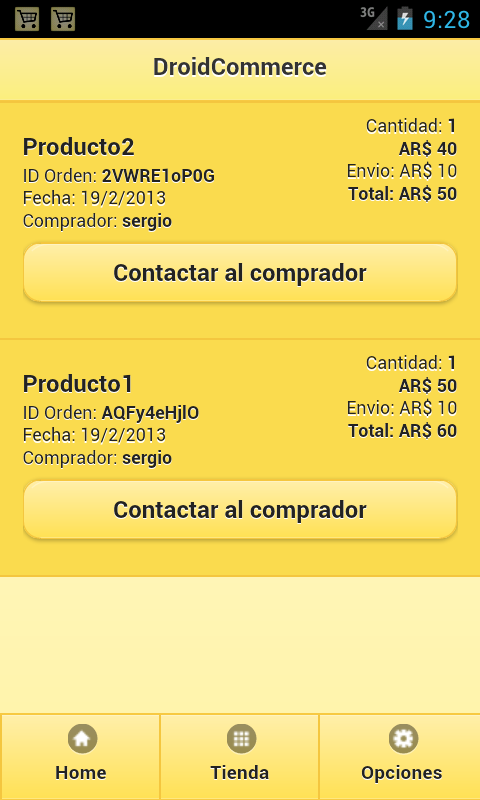
\includegraphics[width=0.6\textwidth]{imagenes/capturas/listado-ventas.png}
        %%Me parece que queda mejor sin el hfill
        %\hfill
        \caption{Pantalla de listado de ventas}
    \label{fig:listado-ventas}
\end{figure}